
\section{Loss functions\label{sec:LossFunctions}}
\par{
    Construction of a machine learning model requires evaluating the model, comparing the result of this evaluation with the desired output and taking steps to make the observed output resemble the desired output better.
    In other words, to train a model, the optimizer will minimize the loss function.
    To use the gradient descent algorithm, this loss function needs to be differentiable.
}
\par{
    Several loss components will be discussed below, both unsupervised and supervised loss functions.
    A supervised loss function component considers the difference between the network prediction and a known (weak) label.
    An unsupervised loss function component considers characteristics of the network output itself. No labels are used in calculating an unsupervised loss component.
    The desirable characteristics that are enforced by the unsupervised loss functions can be part of the \textit{priors}, the knowledge on the problem one has beforehand
    \footnote{To be able to work with weaker, less informative labels, one needs to enter more prior knowledge into the problem}. 
}
In order to make the notation in this section clearer, table \ref{tab:loss_notations} list the notations used in the loss function components.
\begin{SCtable}[\sidecaptionrelwidth][h]
 
    \begin{tabular}{ l l } 
     \hline
     \hline
     Symbol & meaning \\
     \hline 
    $n$                 & Number of problem classes \\
    $X_i$               & Slice $i$ and corresponding context slices   \\ 
    $\vec{p}$           & A pixel position in slice $i$ \\
    $\mathcal{K}$       & Set of outcome classes: $\mathcal{K} = [0, 1, \dots, n-1]$ \\
    $\mathcal{Y}_i$     & set of labels for slice $i$, $\mathcal{Y}_i(\vec{p}) \in \mathcal{K}$  \\
    $\mathcal{I}_i$     & set of pixel positions for which a label is available \\
    $f_\theta(X_i)=z_i$ & model output (logits) for $X_i$ with weights $\theta$. $\vec{z_i(\vec{p})}\in \mathbb{R}^n$ \\
    $\sigma(z_i(\vec{p}))$   & softmax result for $\vec{z_i(\vec{p})}$ ($\in \mathbb{R}^n$ and $\forall k\in \mathcal{K} 0\leq\sigma_k\leq1$) \\
    $w_k$ & A weigth that can be attributed to class $k \in \mathcal{K}$ \\
     \hline
     \hline
    \end{tabular}
    \caption{List of symbols used in the loss functions\label{tab:loss_notations}}

\end{SCtable}
\par{
    In this project, $n=6$ for the coronal and sagittal slice models and $n=2$ for the transverse slice models. 
    Label $\mathcal{Y}_i(\vec{p})=0$ indicates the background class and the lubar vertebrae $L_m$ are indicated with $\mathcal{Y}_i(\vec{p})=m$ ($m\in[1,2,3,4,5]$).
    In the fully supervised case, $\mathcal{I}_i$ spans the complete slice $i$. In the weakly supervised case, there are only a handful of positions $\vec{p}$ for which a label exists.
}
The softmax function $\sigma$ is related to the sigmoid function $\mathbf{S}$. It is defined as:

\begin{eqnarray}
    \sigma_k(z) &=& \frac{\exp(z_k)}{\sum_{m\in\mathcal{K}} \exp(z_m)} \\
    \mathbf{S}(x) &=& \left[ 1+ exp(-x) \right]^{-1} \\ &=& \frac{exp(x)}{exp(x) + 1} 
\end{eqnarray}

The final training loss is given by:
\begin{equation}
    \mathcal{L} = \mathcal{L}_P + \mathcal{L}_E + \mathcal{L}_C + \mathcal{L}_S
\end{equation}
The different loss components are detailed below.

\subsection{Supervised loss functions}

\subsubsection{cross entropy loss \& Point loss \label{sec:crossentropy}}
To compare the network output with the labels, first, the (weighted) cross entropy loss is used\footnote{The weight is optional. One can decide $\forall i\in\mathcal{K}: w_i=1$}.

\begin{equation}
\mathcal{L}_P(X_i) = -\sum_{\vec{p} \in \mathcal{I}_i} w_{\mathcal{Y}_i(\vec{p})}.\log\left[\sigma_{\mathcal{Y}_i(\vec{p})}\left(\vec{z_i(\vec{p})}\right)\right]
\label{eq:LP}
\end{equation}

This loss term is minimized when the network output $z_i(\vec{p})[k]$ with $k=\mathcal{Y}_i(\vec{p})$ the class label for $\vec{p}$ is maximal while the other logits for this position are minimal.
In the fully supervised case, this loss function is called the cross-entropy loss. 
When training a model with point supervision, this is only one of multiple loss components. 
In the case of point supervised data, $\mathcal{I}_i$ only consists of a handful of points.
This loss component is, in this case, called the point loss component $\mathcal{L}_P$.

\subsubsection{Prior extend loss}
The second \Gls{supervisedl} loss function used is the \textit{prior extend} loss.
This loss function describes the prior knowledge that the dimensions of a vertebra are limited. 
Based on \cite{Alam2014}, the maximal extent of a human lumbar vertebrae was set to be $r=110mm$.
This means that a point label $\mathcal{Y}_i(\vec{p})=m: m\in[1,2,3,4,5]$ indicating that $\vec{p}$ is a point in vertebra $L_m$, also means that all points outside of a cicle with radius $r$ cannot be points of $L_m$.
\marginpar{
        % This file was created by tikzplotlib v0.9.8.
\begin{tikzpicture}

\begin{axis}[
height=5cm,
tick align=outside,
width=5cm,
x grid style={white!69.0196078431373!black},
xmin=-0.5, xmax=349.5,
xtick pos=both,
xtick style={color=black},
y dir=reverse,
y grid style={white!69.0196078431373!black},
ymin=-0.5, ymax=349.5,
ytick pos=left,
ytick style={color=black}
]
\addplot graphics [includegraphics cmd=\pgfimage,xmin=-0.5, xmax=349.5, ymin=349.5, ymax=-0.5] {images/prior_extend-000.png};
\addplot [draw=black, fill=black, mark=*, only marks, scatter]
table{%
x  y
120 80
100 35
};
\end{axis}

\end{tikzpicture}

        \captionof{figure}{Illustration of the prior extend mask for annotation points at [120, 80] and [100, 34]. In the grey area, $\mathbf{m} = 0$.}
        \label{fig:prior_extent}
    }
First, $n-1$ (in this case 5) distance masks are created\footnote{1 label is background, for which there is no prior extend.}, 
representing the maximal\footnote{Maximal distance, because there can be mulitple such labels.} distance (Euclidian norm) of each location $\vec{q}$ from the label $\mathcal{Y}_i(\vec{p})=k$ furthest away from $\vec{q}$.
Then $\mathbf{d}$ is converted to a semi-mask:
\begin{eqnarray}
    \mathbf{d}_k(\vec{q}) &=& \max_{\vec{p}:\mathcal{Y}_i(\vec{p})=k}||\vec{q} - \vec{p}||\\
    \mathbf{m}_k(\vec{q}) &=& \mathbf{I}\left( (-\mathbf{d}(\vec{q}) + r) > 0 \right)
\end{eqnarray}
Now, $\mathbf{m}$ is 1 for positions closer than distance $r$ from the points, and it is 0 for positions far from labels with value $k$.
Where $\mathbf{m}_k=0$, the model output should not indicate output class $k$. Where $\mathbf{m}_k=1$, the output class is unknown\footnote{Only channel $k$ is concerned, since one only knows what class these points do not belong to, there is not more information about the other classes.}.

The loss function is the binary cross-entropy between $\mathbf{m}_k$ and the sigmoid of the k$^{th}$ channel of the logits $z_i$ with weight vector $\{1, 0\}$.

\begin{equation}
    \mathcal{L}_E(X_i) = \sum_{k\in\mathcal{K}}\sum_{\vec{q}\in X_i}  (1-\mathbf{m}_k(\vec{q})) \log(\mathbf{S}(z_i(\vec{q})_k)) 
\end{equation}

%\footnote{
%    The cross-entropy loss is easier to interpret when one considers the binary case ($n=2$) over $N$ datapoints with true value $t_i \in \left\{0;1\right\}$ and softmax probability $0 \leq p_i \leq 1$ ($i\in \{0;..;N-1\}$) is defined as 
%\begin{equation}
%    \mathcal{L} = -\frac{1}{N} \left(  
%        \sum^{N-1}_{i=0} \left(
%            t_i log(p_i) + (1 - t_i) log( 1 - p_i )
%        \right)
%     \right)
%\end{equation}}


\subsection{Unsupervised loss functions}

\subsubsection{Transformation consistency loss}
The first \Gls{unsupervisedl} loss function is the unsupervised consistency loss\cite{Laradji2021}. 
The idea behind this loss is that the model output should be consistent for geometric transformations of the input.
A set of geometrical transformations $T=\left\{ t_1, t_2, \dots, t_n \right\}$ is defined. 
Then the consistency loss function $\mathcal{L}_C$ is defined as
\footnote{This function evaluates the difference between the transformation of the model output $t_k\left[f_\theta(X_i)\right]$ and the model output for the transformed input $f_\theta\left( t_k[X_i] \right)$.}
\begin{equation}
    \mathcal{L}_C(X_i) = \sum_{p \in \mathcal{P}_i} \left| t_k\left[f_\theta(X_i)\right]_p - f_\theta\left( t_k[X_i] \right)_p  \right|  
\end{equation}.

In this project, two transformations are combined: rotations of $[90^{\circ}, 180^{\circ}, 270^{\circ}]$ and the horizontal flip.
Each time the loss is called, one transformation $t$ is randomly selected from the list, and the transformation consistency loss is calculated using this transformation.

\subsubsection{Separation loss}
As mentioned when discussing the cross-entropy loss in §\ref{sec:crossentropy}, this loss encourages the model to output the correct label and to decrease the output values for the other labels.
As discussed, the correct label is not known for most of the locations in a weakly supervised problem.
Apart from a limited number of points, there is no such incentive for weakly supervised networks.
For this reason, the separation loss $\mathcal{L}_S$ is introduced.
This loss component consists of the negative sum of the absolute difference of the class segmentation masks\footnote{$z_i[m]$ denotes the $m^{th}$ model output channel.}:
\begin{equation}
    \mathcal{L}_S(X_i) = - \sum_{\vec{p}} \sum_{m\in \mathcal{K}} \sum_{n \in \mathcal{K}, n>m} \mathbf{S}(z_i[m]) - \mathbf{S}(z_i[n])
\end{equation}

This loss component thus provides an incentive to the network to make a decision, even in areas where few annotation points are available.

\begin{SCfigure}[][htb]
\centering
    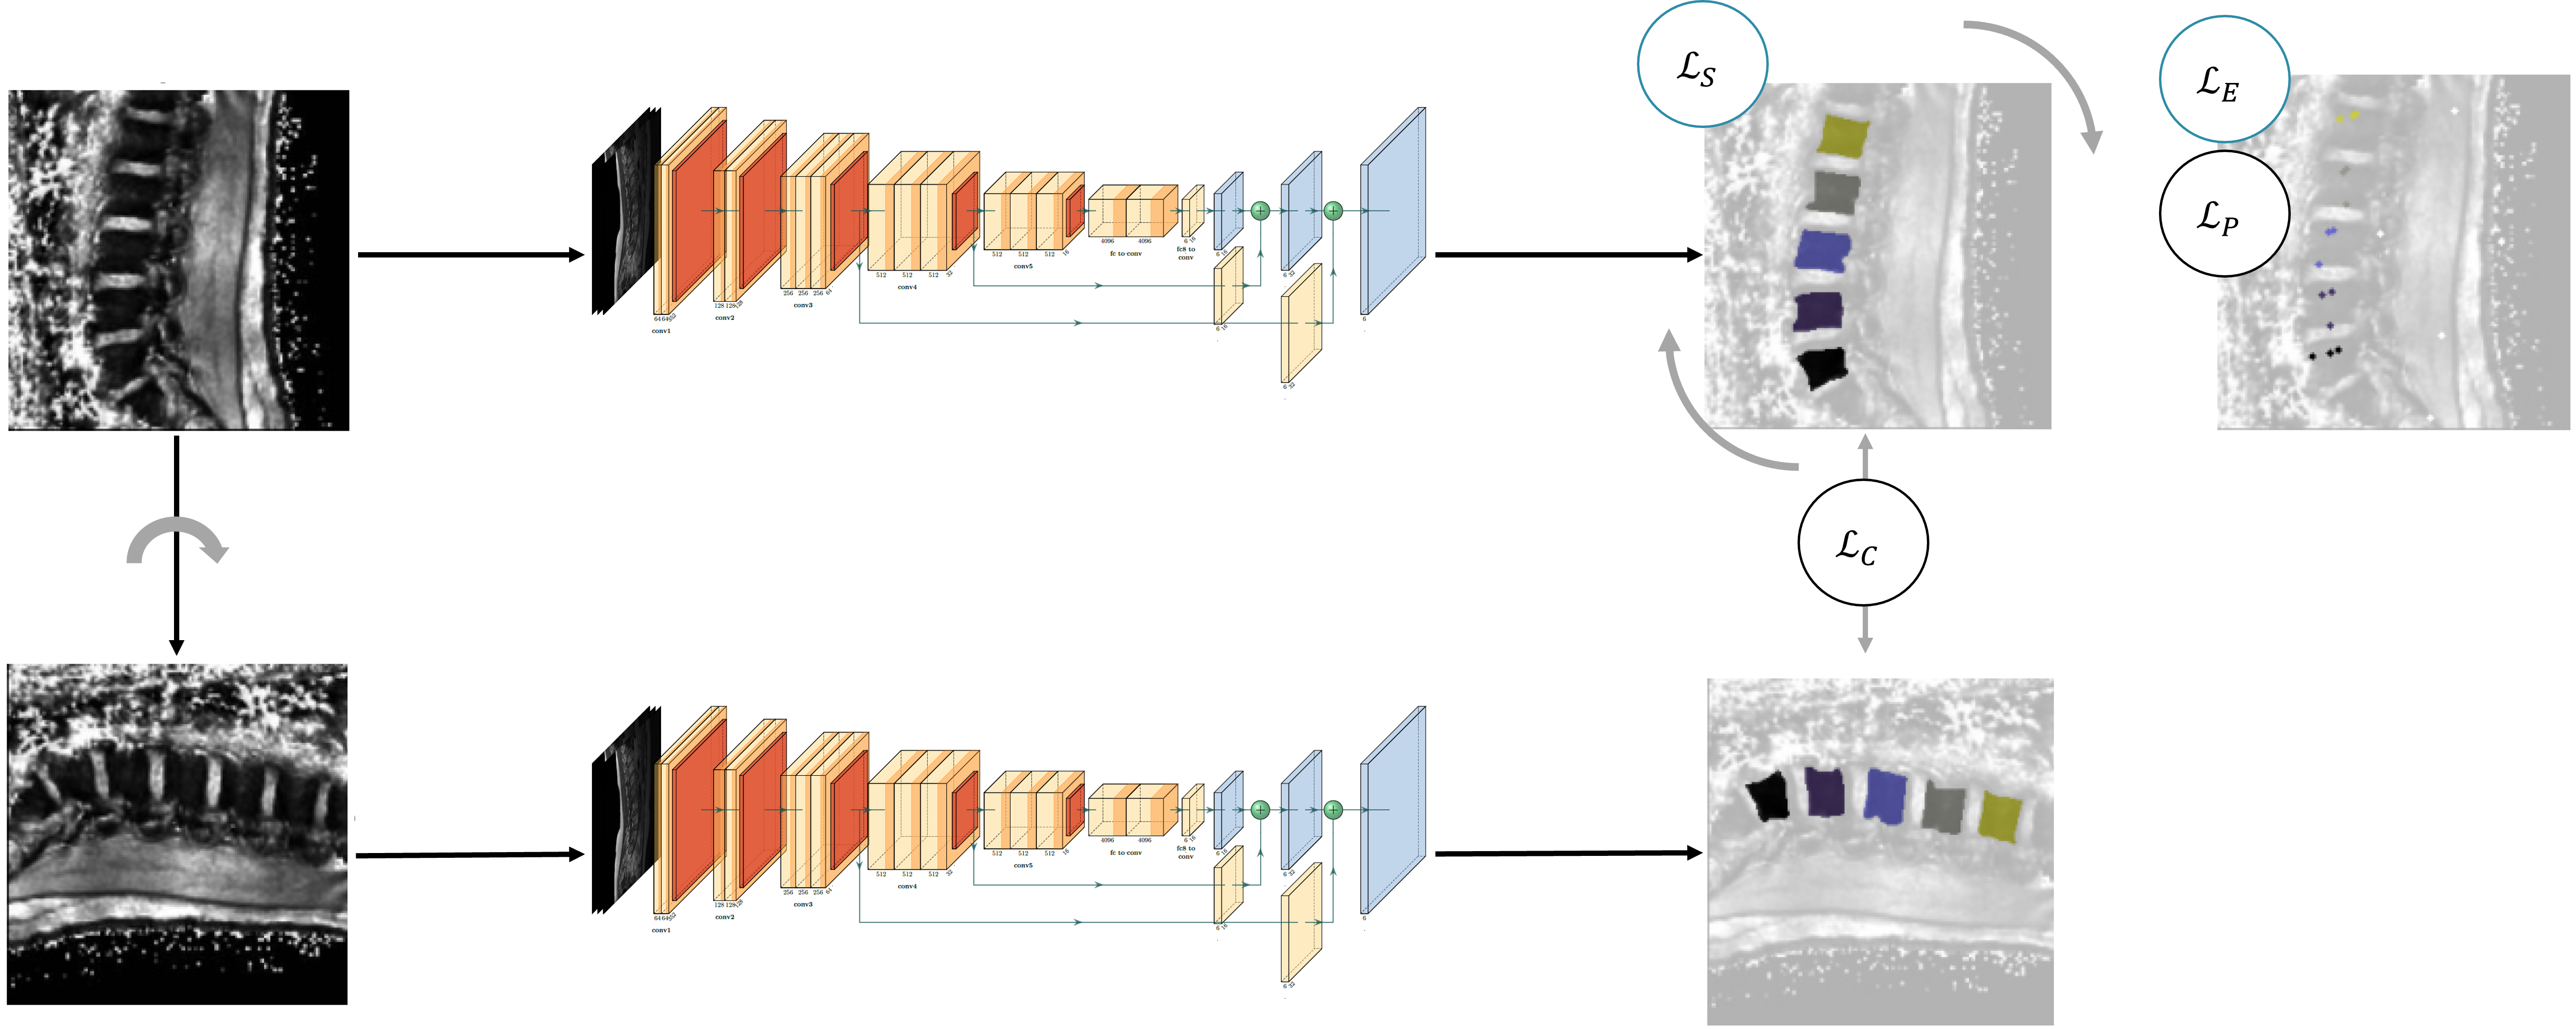
\includegraphics[width=.95\textwidth]{images/Loss_combination.png}
    \caption{Illustration of the loss term combination. The image slice crop is evaluated twice to calculate the consistency loss $\mathcal{L}_C$. For the unsupervised loss terms, only the logits produced by the network are used.
    The supervised loss terms make use of the point annotations.}
\end{SCfigure}